\documentclass[../main.tex]{subfiles}

\begin{document}
\chapter{Stetige Funktionen}

Folgende Definition von Weierstrass
ist aus gutem Grund sehr berühmt.

\begin{definition}
  Sei $A \subset \mathbb{R}$ 
  eine beliebige Teilmenge.
  Eine Funktion
  $f \colon A \to \mathbb{R}$ 
  heisst \emph{stetig} im Punkt
  $p \in A$, falls für
  alle vorgegebenen $\varepsilon > 0$
  ein  $\delta > 0$ existiert,
  so dass für alle $q \in A$ 
  mit $|q-p| \leq \delta$ gilt,
  dass $|f(q) - f(p)| \leq \varepsilon$.
  Falls $f \colon A \to \mathbb{R}$ in
  allen Punkten $p \in A$ stetig ist,
  dann heisst $f$ \emph{stetig}.
\end{definition}

\begin{figure}[htb]
  \centering
  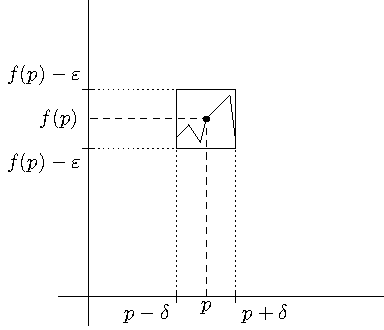
\includegraphics{chapter3/images/conti}
  \caption{Stetigkeit}%
  \label{fig:conti}
\end{figure}


\begin{examples}
  \leavevmode
  \begin{enumerate}[(1)]
    \item Die Identitätsfunktion
      \begin{align*}
        f \colon \mathbb{R} & \to \mathbb{R} \\
        p & \mapsto p
      \end{align*}
      ist stetig. Sei dazu $p \in \mathbb{R}$ fest
      und $\varepsilon > 0$ vorgegeben.
      Setze $\delta = \varepsilon$. Dann gilt
      für alle $q \in \mathbb{R}$ mit
      $|q - p| \leq \delta$, dass
      $|f(q) - f(p)| = |q - p| \leq \delta = \varepsilon$.
    \item Sei
      \[
        f(x) = 
        \begin{cases}
          0 & \text{falls } x \leq 0, \\
          1 & \text{falls } x > 0,
        \end{cases}
      \]
      siehe Abbildung~\ref{fig:jump}.
      Dann ist $f$ in allen Punkten ausser dem
      Nullpunkt stetig.
      Tatsächlich, sei $p \neq 0$
      und $\varepsilon > 0$ 
      vorgegeben.
      Setze $\delta = |p|/2 > 0$.
      Dann gilt für alle $q \in \mathbb{R}$ 
      mit $|q - p| \leq \delta$, dass
      $|f(q) - f(p)| = 0 \leq \varepsilon$.
      
      Sei nun $p = 0$. Betrachte $\varepsilon = 1/2$.
      Sei $\delta > 0$ beliebig.
      Dann gilt für $q = \delta/2$, dass
      $|q - p| = \delta/2 < \delta$.
      Es folgt
      \[
        |f(q) - f(p)| = |1 - 0| = 1 > \varepsilon.
      \]
      \begin{figure}[htb]
        \centering
      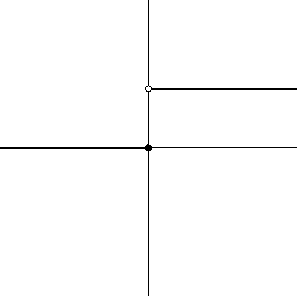
\includegraphics{chapter3/images/jump}
        \caption{Sprungstelle}%
        \label{fig:jump}
      \end{figure}

    \item Sei
      \[
        f(x) = 
        \begin{cases}
          1, & \text{falls } x \in \mathbb{Q}, \\
        0,& \text{falls } x \in \mathbb{R} \setminus \mathbb{Q}
        \end{cases}
      \]
      die \emph{Dirichletfunktion}.
      Dann ist $f$ in keinem Punkt stetig.
      Betrachte dazu $\varepsilon = 1/2$.
      Sei $p \in \mathbb{Q}$, das heisst $f(p) = 1$.
      Für alle $\delta > 0$ finden wir eine
      irrationale Zahl
      $q \in \mathbb{R} \setminus \mathbb{Q}$ mit
      $|q - p| \leq \delta$ 
      und
      $|f(q) - f(p)| = 1 > \varepsilon$.
      Tatsächlich, wähle $N \in \mathbb{N}$ 
      mit $\sqrt 2 / N \leq \delta$.
      Setze
      $q = p +\sqrt 2/N$. Dann gilt  $q \notin \mathbb{Q}$,
      also $f(q) = 0$.

      Analog, sei $p \in \mathbb{R} \setminus \mathbb{Q}$,
      das heisst $f(p) = 0$.
      Für alle $\delta > 0$ finden wir
      eine Zahl $q \in \mathbb{Q}$ mit $|q - p| \leq \delta$ 
      und
      $|f(q) - f(p)| = 1 > \varepsilon$.
      Tatsächlich,
      wähle $N \in \mathbb{N}$ mit $1/N \leq \delta$.
      Dann existiert $a \in \mathbb{Z}$
      so dass
      $|a/N - p| \leq 1/N$.
      Setze $q = a/N$.
    \item Sei $f(x) = x^n$ für $n \in \mathbb{N}$.
      Dann ist $f$ stetig auf $\mathbb{R}$.
      Sei also $p \in \mathbb{R}$ vorgegeben und
      sei $\varepsilon > 0$.
      Für
      $h \in \mathbb{R}$ mit $|h| \leq 1$ gilt
      \[
        f(x + h) = (x + h)^n = \sum_{k=0}^{n} \binom{n}{k}
        x^{n-k}h^k
        = x^n + nx^{n-1}h + \frac{n(n-1)}{2}x^{n-2}h^2 + \cdots.
      \]
      Es folgt, dass
      \[
        |f(x + h) - f(x)| \leq |h| \cdot
        \left| \sum_{k=1}^{n} \binom{n}{k} x^{n-k} \right|,
      \]
      da $|h| \leq 1$.
      Setze jetzt
      \[
        \delta_1 = \frac{\varepsilon}{t+1},
      \]
      wobei
      \[
        t = \sum_{k=1}^{n} \binom{n}{k} |p|^{n-k},
      \]
      und $\delta = \min \{1, \delta_1\} > 0$.
      Für alle  $h \in \mathbb{R}$
      mit $|h| \leq \delta$ gilt also
      \[
        |f(p+h) - f(p)| \leq |h| \cdot t \leq
        \delta_1 \cdot t = \varepsilon \cdot \frac{t}{t+1}
        \leq \varepsilon.
      \]
      Also ist $f$ stetig im Punkt $p$.
    \item Betrachte die Funktion
      \begin{align*}
        f \colon \mathbb{R} \setminus \{0\} & \to \mathbb{R} \\
        x & \mapsto 1/x.
      \end{align*}
      Dann ist $f$ stetig in allen Punkten
      $p \in \mathbb{R} \setminus \{0\}$. Dies ist
      mühsam von Hand zu zeigen. Deshalb
      verwenden wir folgendes Lemma.
  \end{enumerate}
\end{examples}

\begin{lemma*}
  Sei $A \subset \mathbb{R}$ und seien
  $f, g \colon A \to \mathbb{R}$ im Punkt
  $p \in A$ stetig. Dann sind die Funktionen
  $f + g$ und $f \cdot g$ 
  im Punkt $p$ stetig.
  Falls $f(p) \neq 0$, dann
  existiert $a > 0$, so dass
  die Funktion $1/f$ auf der Menge
  $(p- a, p + a) \cap A$ definiert und 
  im Punkt $p$ stetig ist.
\end{lemma*}

\begin{proof}
  Als erstes zeigen wir,
  dass $f  + g$ stetig ist.
  Sei $\varepsilon > 0$ vorgegeben.
  Wähle $\delta_f > 0$ und  $\delta_g > 0$ 
  so dass für alle $q \in A$ mit
  $|q - p| \leq \delta_f$ gilt, dass
  $|f(q) - f(p)| \leq \varepsilon/2$,
  und so dass für alle
  $q \in A$ mit $|q - p| \leq \delta_g$ 
  git, dass
  $|g(p) - g(q)| \leq \varepsilon/2$.
  Setze $\delta = \min \{\delta_f, \delta_g\}$.
  Dann gilt für alle $q \in A$ mit
  $|q - p| \leq \delta$, dass
  \begin{align*}
  |(f + g)(q) - (f + g)(p)| &     = |f(q) + g(q) - f(p) - g(p)|\\
                            & \leq |f(q) - f(p)| + |g(q) - g(p)|\\
                            & \leq \varepsilon/2 + \varepsilon/2\\
                            &= \varepsilon.
  \end{align*}

  Wir zeigen nun, dass $f \cdot g$ stetig ist.
  Berechne
  \begin{align*}
     |(f\cdot g)(q) - (f \cdot g)(p)|
     & = |f(q) \cdot g(q) - f(p) \cdot g(p)| \\
     & = |f(q)g(q) - f(p)g(q) + f(p)g(q) - f(p) g(p)| \\
     & \leq |g(q)| \cdot |f(q) - f(p)| + 
     |f(p)| \cdot |g(q) - g(p)| \\
  \end{align*}
  Wähle $\delta_1 > 0$ so, dass immer wenn
  $|q - p| \leq \delta_1$ gilt, dann auch
  $|g(q) - g(p)| \leq 1$. Wähle
  $\delta_2 > 0$ so, dass immer
  wenn $|q - p| \leq \delta_2$ gilt, dann auch
  \[
    |f(q) - f(p)| \leq \frac{\varepsilon}{2} \cdot
    \frac{1}{|g(p)| + 1}.
  \]
  Wähle weiterhin $\delta_3 > 0$ so, dass immer wenn
  $|q - p| \leq \delta_3$ gilt, dann auch
  \[
    |g(q) - g(p)| \leq \frac{\varepsilon}{2} \cdot
    \frac{1}{|f(p)| + 1}.
  \]
  Setze $\delta = \min \{\delta_1, \delta_2, \delta_3 \}$.
  Für $q \in A$ mit $|q - p| \leq \delta$ gilt dann:
  \begin{align*}
    |(f \cdot g)(q) - (f \cdot g)(p)
    &\leq |g(q)| \cdot \frac{\varepsilon}{2} \cdot  
    \frac{1}{|g(p)| + 1}
    + |f(p)| \cdot \frac{\varepsilon}{2}
    \cdot \frac{1}{|f(p)| + 1}\\
    & \leq (|g(p)| + 1) \frac{\varepsilon}{2}
    \cdot \frac{1}{|g(p)| + 1} + \frac{\varepsilon}{2}  \\
    &= \varepsilon.
  \end{align*}
  
  Zuletzt behandeln wir $1/f$.
  Sei $p \in A$ mit $f(p) \neq 0$.
  Dann existiert nach Stetigkeit von
  $f$ im Punkt $p$ eine Zahl $a > 0$, so dass
  wenn $|q - p| \leq a$ gilt,
  dann auch
  \[
  |f(q) - f(p)| \leq \frac{|f(p)|}{2}.
  \]
  Also ist $1/f$ auf der Menge $(p-a, p+a) \cap A$ definiert,
  da dort $|f(q)| > 0$.
  Sei nun $\varepsilon > 0$. 
  Berechne
   \begin{align*}
     \left| \frac{1}{f(q)} - \frac{1}{f(p)} \right| 
     & = \left| \frac{f(p) - f(q)}{f(q)f(p)} \right| \\
     & \leq 2 \cdot \frac{|f(p) - f(q)|}{|f(p)|^2}. 
  \end{align*}
  Wähle $\delta > 0$, so dass $\delta \leq a$ 
  und immer wenn $|q - p| \leq \delta$,
  dann auch 
  \[
    |f(q) - f(p)| \leq \frac{\varepsilon}{2} \cdot |f(p)|^2.
  \]
  Es folgt für $q \in A$ mit $|q - p| \leq \delta$, dass
  \[
    \left| \frac{1}{f(q)}- \frac{1}{f(p)} \right|
    \leq 2 \cdot \frac{|f(p) - f(q)|}{|f(p)|^2} \leq \varepsilon.
    \qedhere
  \]
\end{proof}

\begin{applications}
  \leavevmode
  \begin{enumerate}[(1)]
    \item Alle Funktionen der Form
      \[
        f(x) = a_n x^n + a_{n-1} x^{n-1} + \cdots + a_{1} x + a_0,
      \]
      sogenannte \emph{Polynome},
      mit Koeffizienten $a_k \in \mathbb{R}$ sind stetig
      auf $\mathbb{R}$, da die Funktion $x \mapsto x$
      und konstante Funktionen stetig sind.
    \item Die Funktion $f(x) = 1/x$ ist stetig
      auf $\mathbb{R} \setminus \{0\}$.
  \end{enumerate}
\end{applications}

\subsection*{Folgenstetigkeit}
\begin{theorem}
  Sei $A \subset \mathbb{R}$ eine Teilmenge.
  Eine Funktion $f \colon A \to \mathbb{R}$ ist
  genau dann stetig im Punkt
  $p \in A$, wenn für alle
  konvergenten Folgen $a \colon \mathbb{N} \to A$
  mit $\lim_{n \to \infty}a_n = p$ gilt, dass
  \[
    \lim_{n \to \infty} f(a_n) = f(p).
  \]
\end{theorem}

\begin{proof}
  Für die Hinrichtung ``$\Rightarrow$'' sei $f$
  im Punkt $p$ stetig. Sei ${(a_{n})}_{n \in \mathbb{N}}$ 
  eine Folge in $A$ mit
  \[
    \lim_{n \to \infty} a_n = p.
  \]
  Sei $\varepsilon > 0$ vorgegeben.
  Dann existiert $\delta > 0$ so dass immer wenn
  $|q - p| \leq \delta$, dann auch
  $|f(q) - f(p)| \leq \varepsilon$.
  Wähle $N \in \mathbb{N}$, so
  dass für $n \in \mathbb{N}$ mit $n \geq N$ gilt,
  dass $|a_n - p| \leq \delta$.
  Es gilt also für $n \geq N$, dass
  $|f(a_n) - f(p)| \leq \varepsilon$.
  Also gilt
  \[
    \lim_{n \to \infty} f(a_n) = f(p).
  \]
  
  Für die Rückrichtung ``$\Leftarrow$'', nehme an,
  dass $f$ ``folgenstetig'' in $p$ ist,
  das heisst dass für alle
  konvergenten Folgen $a \colon \mathbb{N} \to A$
  mit $\lim_{n \to \infty} a_n = p$ gilt,
  dass
  \[
    \lim_{n \to \infty} f(a_n) = f(p).
  \]
  Wir beweisen durch Widerspruch, dass
  $f$ stetig in $p$ ist.
  Nehme an, dass $f$ nicht stetig in $p$ ist.
  Dann existiert $\varepsilon_0 > 0$, so dass
  für alle $\delta > 0$ ein $q \in A$ 
  existiert, so dass
  $|q - p| \leq \delta$ und $|f(q) - f(p)| > \varepsilon_0$.
  Wähle nun eine Folge
  ${(a_{n})}_{n \in \mathbb{N}}$ wie folgt.
  Wähle $a_n \in A$ so dass
  $|a_n - p| \leq 1/(n+1)$ und $|f(a_n) - f(p)| > \varepsilon_0$.
  Nach Konstruktion gilt
  $\lim_{n \to \infty} a_n = p$, aber
  \[
    \lim_{n \to \infty} f(a_n) \neq f(p).
  \]
  Dies widerspricht der Folgenstetigkeit von $f$.
\end{proof}




\end{document}
